\chapter{Backtracking Algorithms}\label{chap:backtracking}
\section{Thinking in Backtracking Algorithms}
{\color{blue}{Backtracking algorithms}} are a systematic way to search or traverse all the potential solutions in the solutions space. \\

Backtracking algorithms go through all the {\color{blue}{partial solutions}} that could be {\color{blue}{incrementally}} {\color{blue}{completed}} to give the final solutions. The {\color{blue}{partial solutions}} are represented as the {\color{blue}{nodes}} of a {\color{ForestGreen}{\ul{potential search tree}}}. Each {\color{blue}{partial solution}} is the parent of the {\color{blue}{partial solutions}} that differ from it by a single {\color{blue}{extension step}}, which is represented by an {\color{blue}{edge}}; the {\color{blue}{leaves}} of the tree are the {\color{blue}{partial solutions}} that cannot be extended any further. The {\color{blue}{depth of a node}} represents the {\color{blue}{level of recursion}}.\\

{\color{blue}{Backtracking algorithms}} traverse this {\color{blue}{potential search tree}} {\color{blue}{recursively}}, {\color{blue}{from the root down}}, in {\color{blue}{depth-first order}}. At each node {\colorbox{CodeBackground}{\lstinline|c|}}, the algorithm checks whether {\colorbox{CodeBackground}{\lstinline|c|}} can be completed to a valid solution. If it cannot, the whole sub-tree rooted at {\colorbox{CodeBackground}{\lstinline|c|}} is skipped ({\color{blue}{pruned}}). Otherwise, the algorithm 1) checks whether {\colorbox{CodeBackground}{\lstinline|c|}} itself is a valid solution, and if so reports it to the user; 2) recursively enumerates all sub-trees of {\colorbox{CodeBackground}{\lstinline|c|}}. \\

The {\color{ForestGreen}{\ul{potential search tree}}} has the same structure as the {\color{ForestGreen}{\ul{activation tree}}}. Both trees essentially serve to illustrate how backtracking algorithms solve the problem. The key difference lies in their perspectives. The {\color{blue}{potential search tree}} gives us a {\color{blue}{high-level, problem-oriented view}}, showing how we explore all the partial solutions. On the other hand, the {\color{blue}{activation tree}} provides a more {\color{blue}{low-level, execution-oriented view}}, detailing the steps the algorithm actually takes during its execution.

\subsection{Recursion, Backtracking, and DFS}
Refer to \hyperref[subsec:recursion_backtracking_dfs]{Recursion, Backtracking, and DFS}.

\subsection{How to identify backtracking problems?}
Backtracking algorithms are designed for searching for traversing potential solutions in a space. These solutions are systematically generated by incrementally building upon partial solutions. \\

In practical, there are several typical kinds of problems that can be solved by backtracking algorithms:
\begin{itemize}
	\item {\color{blue}{Combination}} and {\color{blue}{Permutation}} Problem
	\item {\color{blue}{Subset}} Problem
	\item {\color{blue}{Rod Cutting}} Problem
	\item Board Game Problem
\end{itemize}

\subsection{Steps to solve backtracking problems}
The key part is to build the {\color{blue}{potential search tree}}, where the {\color{blue}{nodes}} represent {\color{blue}{partial solutions}} and {\color{blue}{edges}} represent {\color{blue}{extension steps}}. Once the correct {\color{blue}{potential search tree}} is established, you already know how the recursion works.\\

Practical tips:
\begin{itemize}
	\item Backtracking algorithms are a kind of recursion, so the steps of designing a recursive algorithm (\ref{subsec:steps_to_design_recursive_algorithms}) also apply here.
	\item {\color{blue}{Searching order}} should be preset to ensure that each potential solution in the space is visited exactly once.
\end{itemize}

\section{LC 0077 - Combinations}
Given two integers {\colorbox{CodeBackground}{\lstinline|n|}} ({\colorbox{CodeBackground}{\lstinline|n >= 1|}}) and {\colorbox{CodeBackground}{\lstinline|k|}} ({\colorbox{CodeBackground}{\lstinline|k >= 1|}}), return all \ul{combinations} of {\colorbox{CodeBackground}{\lstinline|k|}} numbers chosen from the range {\colorbox{CodeBackground}{\lstinline|[1, n]|}}.\\

You may return the answer in any order. \\

Examples:
\begin{itemize}
	\item {\colorbox{CodeBackground}{\lstinline|n = 4, k = 2 --> [[1,2],[1,3],[1,4],[2,3],[2,4],[3,4]]|}}
	\item {\colorbox{CodeBackground}{\lstinline|n = 1, k = 1 --> [[1]]|}}
\end{itemize}

\subsection*{Solution - Backtracking}
\begin{lstlisting}
std::vector<std::vector<int>> combine(int n, int k) {
	std::vector<std::vector<int>> solutions;
	std::vector<int> comb;
	Backtracking(n, k, 1, comb, solutions);
	return solutions;
}

void Backtracking(int n, int k, int start, std::vector<int>& comb,
								  std::vector<std::vector<int>>& solutions) {
	// valid solution (base case)
	if (k == 0) {
		solutions.push_back(comb);
		return;
	}
	for (int i = start; i <= n; ++i) {
		comb.push_back(i);
		Backtracking(n, k - 1, i + 1, comb, solutions);
		comb.pop_back();
	}
}

\end{lstlisting}\mbox{}

In the case of {\colorbox{CodeBackground}{\lstinline|n = 4|}} and {\colorbox{CodeBackground}{\lstinline|k = 2|}}, the {\color{blue}{potential search tree}} is as follows. 

\begin{figure}[H]
	\centering
	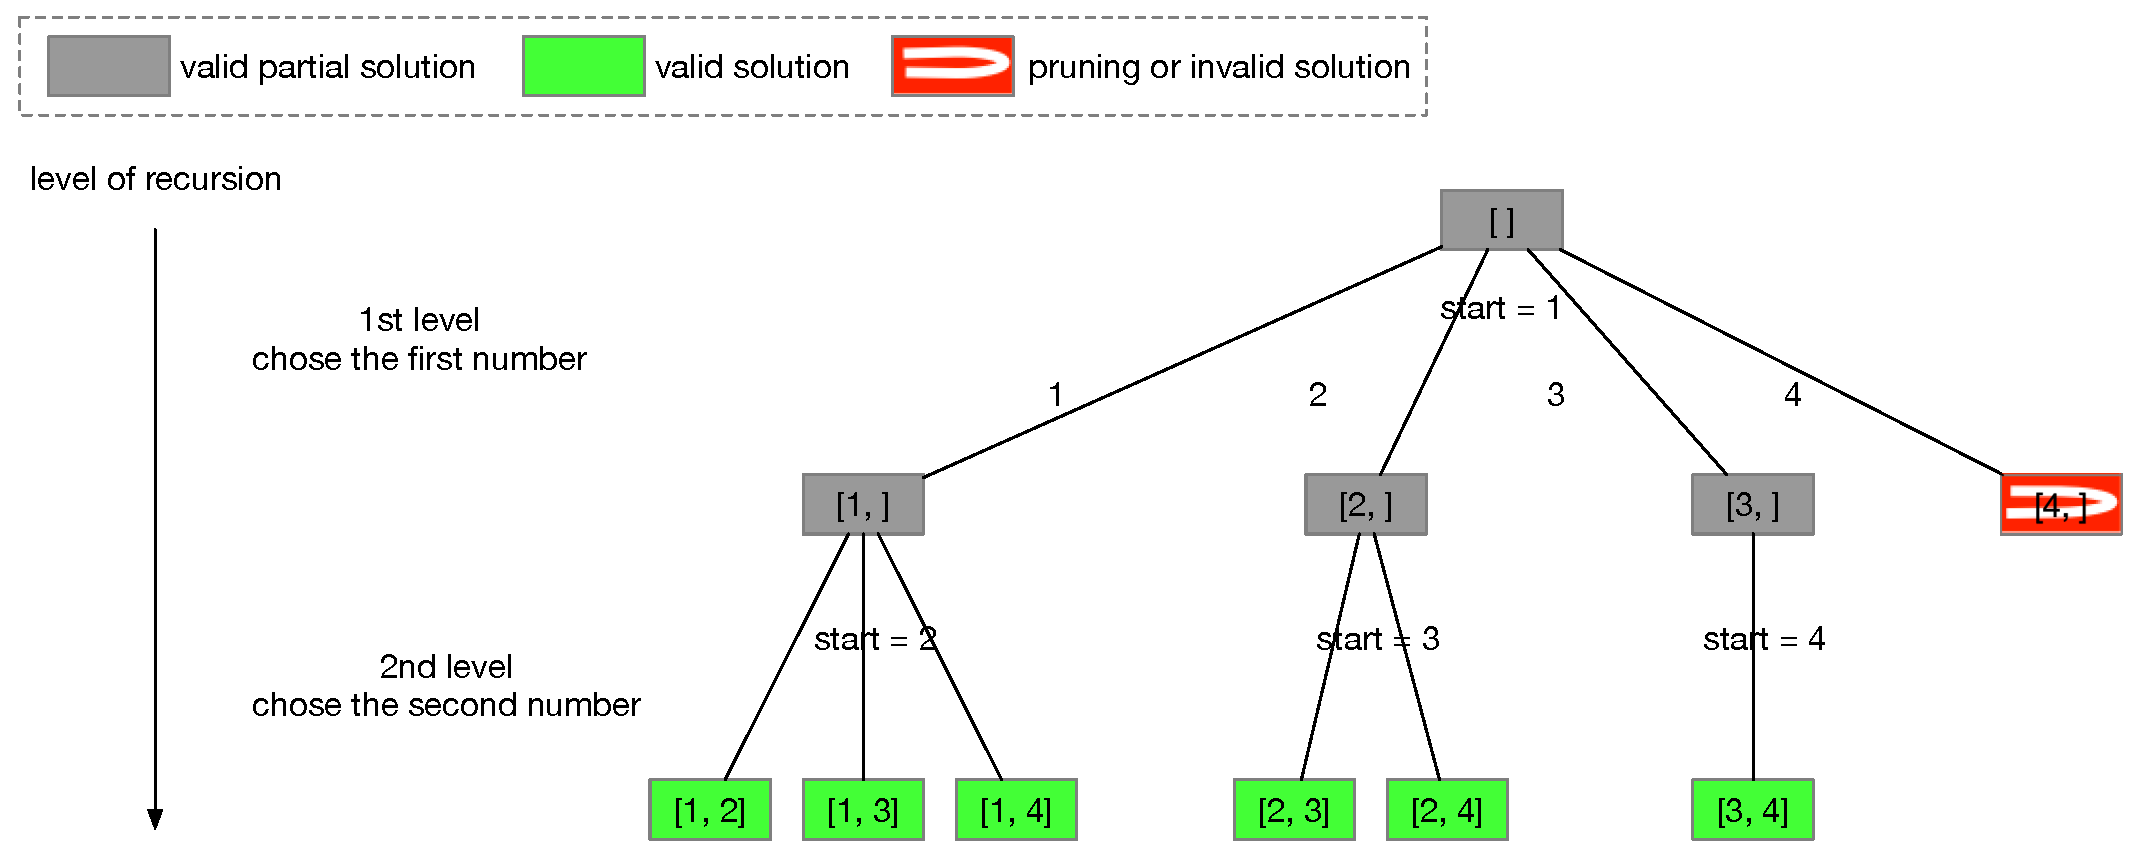
\includegraphics[width=1.0\linewidth]{images/lc0077_pst}
	\label{fig:lc0077pst}
\end{figure}

The {\color{blue}{search order}} is implicitly set via {\colorbox{CodeBackground}{\lstinline|start|}} to ensure that each potential solution is visited exactly once.

\section{LC 0017 - Letter Combinations of a Phone Number}
Given a string containing digits from {\colorbox{CodeBackground}{\lstinline|`2'-`9'|}}, return all possible letter \ul{combinations} that the number could represent. \\

A mapping of digits to letters (just like on the telephone buttons) is given below. Note that {\colorbox{CodeBackground}{\lstinline|`0'|}} and {\colorbox{CodeBackground}{\lstinline|`1'|}} do not map to any letters and {\colorbox{CodeBackground}{\lstinline|digits|}} does not include them neither.

\begin{figure}[H]
	\centering
	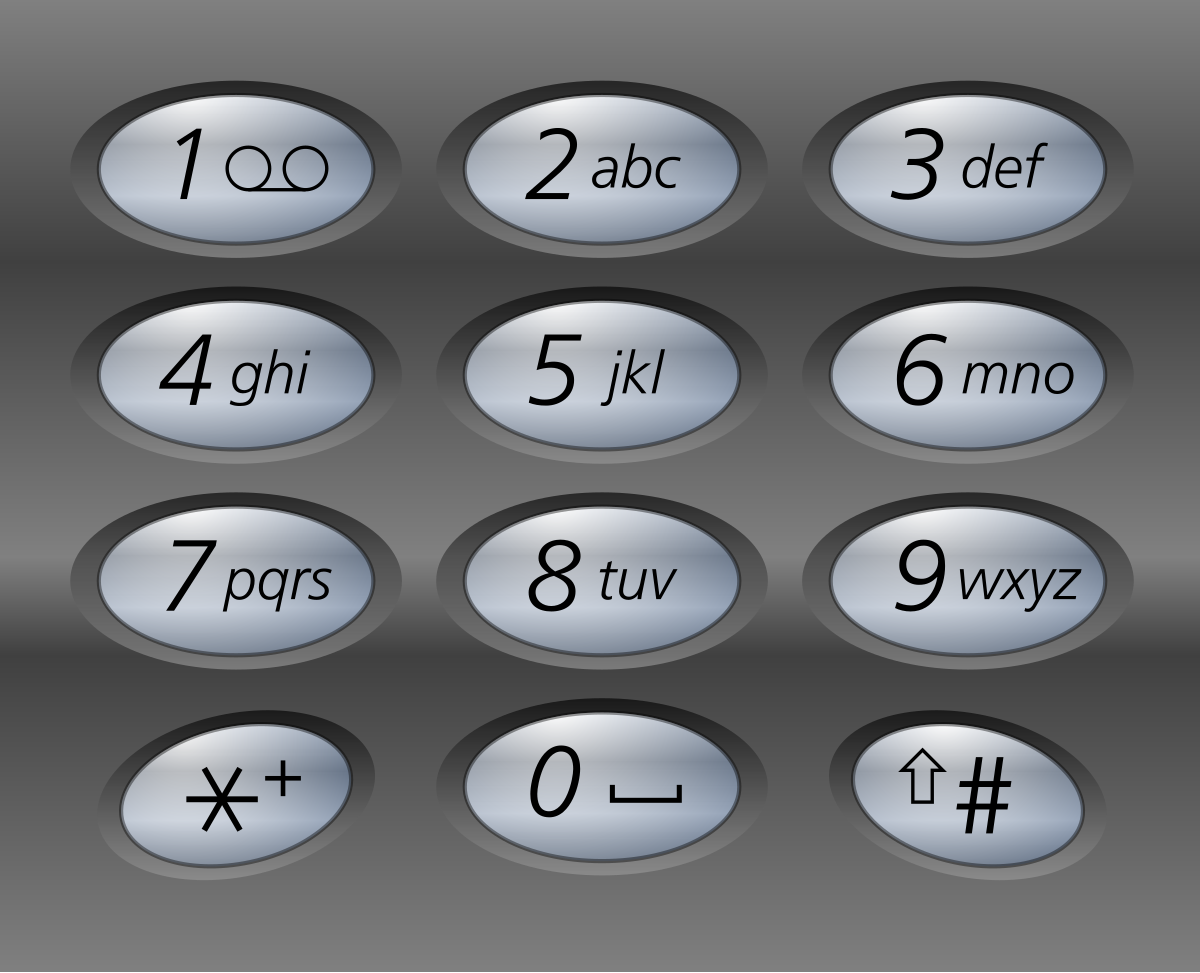
\includegraphics[width=0.3\linewidth]{images/lc0029}
	\label{fig:lc0029}
\end{figure}

You may return the answer in any order.\\

Examples:
\begin{itemize}
	\item {\colorbox{CodeBackground}{\lstinline|digits="23" --> ["ad","ae","af","bd","be","bf","cd","ce","cf"]|}}
	\item {\colorbox{CodeBackground}{\lstinline|digits="" --> []|}}
	\item {\colorbox{CodeBackground}{\lstinline|digits="2" --> ["a","b","c"]|}}
\end{itemize}

\subsection*{Solution - Backtracking}
\begin{lstlisting}
std::vector<std::string> letterCombinations(std::string digits) {
	if (digits.empty()) { return {}; }
	std::string str;
	std::unordered_map<char, std::string> digit2letters = 
	{{'2', "abc"}, {'3', "def"}, {'4', "ghi"},
		{'5', "jkl"}, {'6', "mno"}, {'7', "pqrs"},
		{'8', "tuv"}, {'9', "wxyz"}};
	std::vector<std::string> solutions;
	Backtracking(digits, 0, digit2letters, str, solutions);
	return solutions;
}

void Backtracking(const std::string& digits, int idx,
								  const std::unordered_map<char, std::string>& digit2letters, 
								  std::string& str, std::vector<std::string>& solutions) {
	// valid solution (base case)
	if (idx == digits.size()) {
		solutions.push_back(str);
		return;
	}
	const std::string& letters = digit2letters.at(digits[idx]);
	for (char letter : letters) {
		str.push_back(letter);
		Backtracking(digits, idx + 1, digit2letters, str, solutions);
		str.pop_back();
	}
}
\end{lstlisting}\mbox{}

In the case of {\colorbox{CodeBackground}{\lstinline|dignts = "23"|}}, the {\color{blue}{potential search tree}} is as follows. \\

It should be noted that the {\color{blue}{search order}} is implicitly set to ensure that each potential solution is visited exactly once.
\begin{figure}[H]
	\centering
	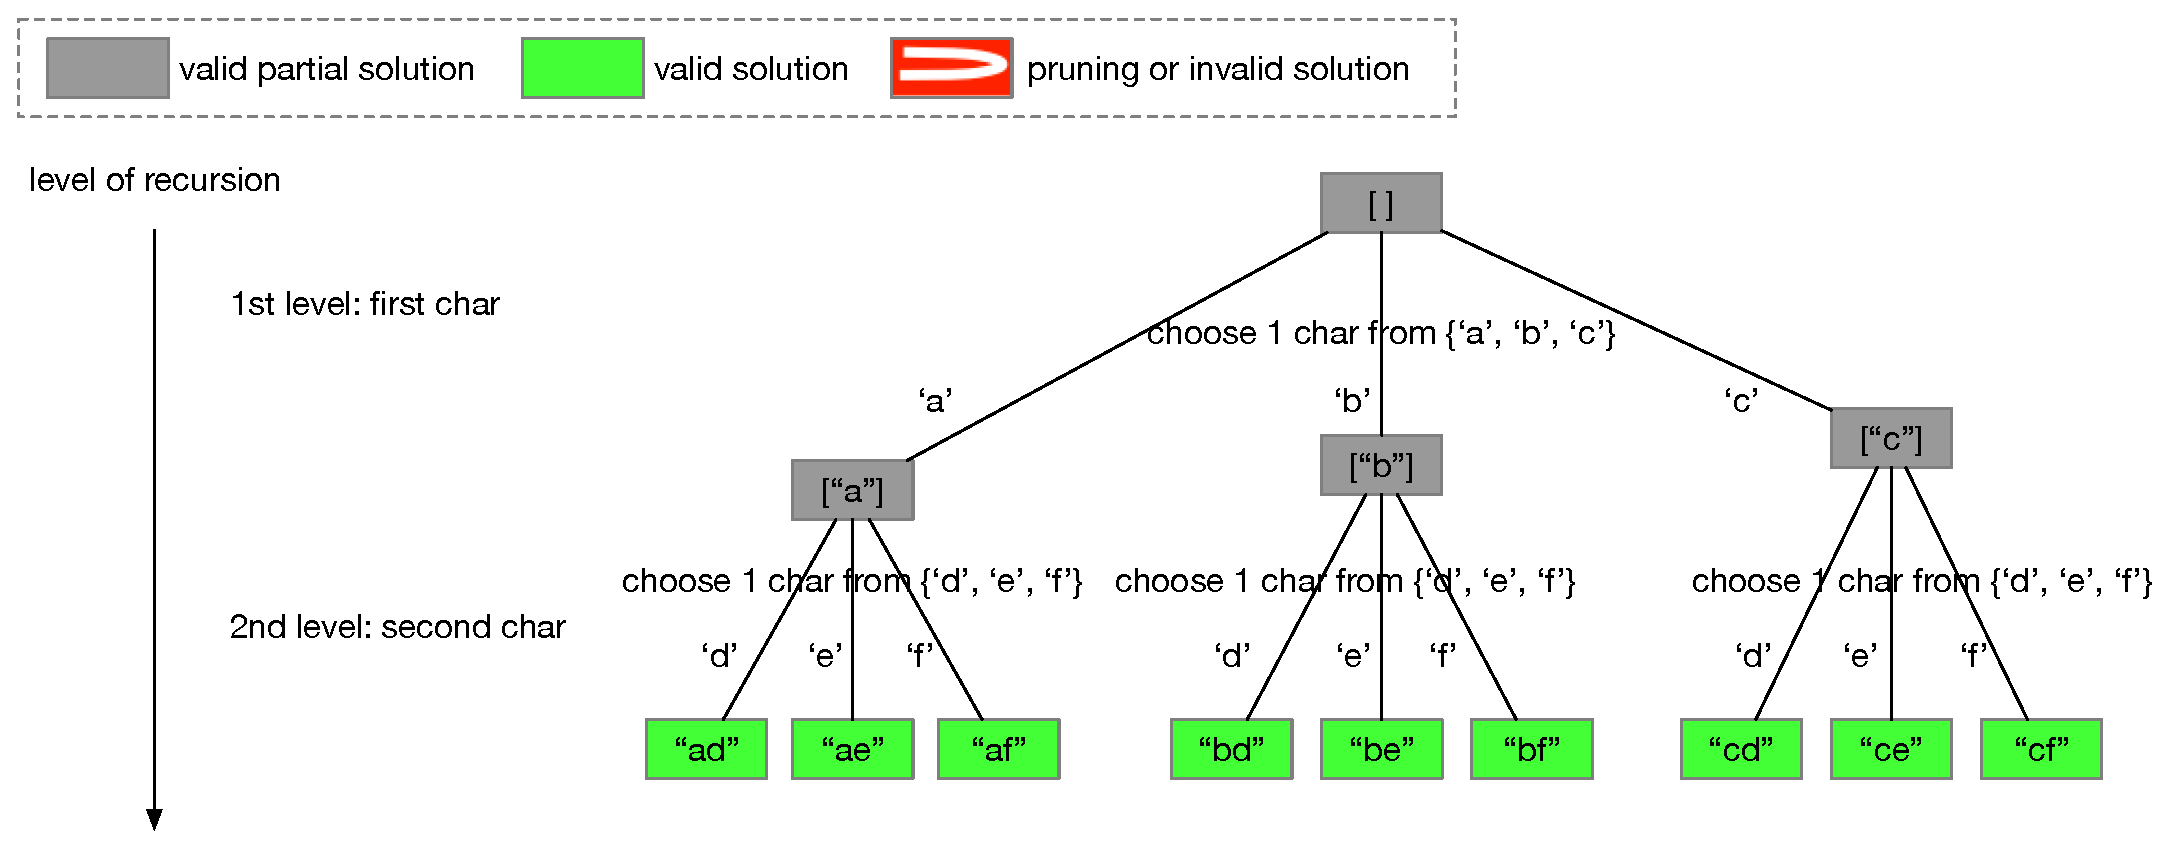
\includegraphics[width=1.0\linewidth]{images/lc0017_pst}
	\label{fig:lc0017pst}
\end{figure}

\section{LC 0039 - Combination Sum}\label{lc0039}
Given a \ul{non-empty} \ul{array} of \ul{distinct integers} {\colorbox{CodeBackground}{\lstinline|candidates|}} ({\colorbox{CodeBackground}{\lstinline|candidates[i] >= 2|}}) and a \ul{target integer} {\colorbox{CodeBackground}{\lstinline|target|}} ({\colorbox{CodeBackground}{\lstinline|target >= 1|}}), return a list of all \ul{combinations} of integers in {\colorbox{CodeBackground}{\lstinline|candidates|}} that add up to {\colorbox{CodeBackground}{\lstinline|target|}}.\\

Each number in {\colorbox{CodeBackground}{\lstinline|candidates|}} may be used \ul{an unlimited number of times} in the combination.\\

You may return the combinations in any order.\\

Examples:
\begin{itemize}
	\item {\colorbox{CodeBackground}{\lstinline|candidates = [2,3,6,7], target = 7 --> [[2,2,3],[7]]|}}
	\item {\colorbox{CodeBackground}{\lstinline|candidates = [2,3,5], target = 8 --> [[2,2,2,2],[2,3,3],[3,5]]|}}
	\item {\colorbox{CodeBackground}{\lstinline|candidates = [2], target = 1 --> []|}}
\end{itemize}

\subsection*{Solution 1 - Backtracking}
\begin{lstlisting}
std::vector<std::vector<int>> combinationSum(std::vector<int>& candidates, int target) {
	std::vector<std::vector<int>> solutions;
	std::vector<int> comb;
	Backtracking(candidates, target, 0, comb, solutions);
	return solutions;
}

void Backtracking(const std::vector<int>& candidates, int target, int start, 
								  std::vector<int>& comb, std::vector<std::vector<int>>& solutions) {
	// valid solution (base case)
	if (target == 0) {
		solutions.push_back(comb);
		return;
	}
	for (int i = start; i < candidates.size(); ++i) {
		// pruning
		if (candidates[i] > target) { continue; }
		comb.push_back(candidates[i]);
		Backtracking(candidates, target - candidates[i], i, comb, solutions);
		comb.pop_back();
	}
}
\end{lstlisting}\mbox{}

In the case of {\colorbox{CodeBackground}{\lstinline|candidates = [2, 3 ,6, 7]|}} and {\colorbox{CodeBackground}{\lstinline|target = 7|}}, the {\color{blue}{potential search tree}} is as follows. \\

It should be noted that the {\color{blue}{search order}} is implicitly set to ensure that each potential solution is visited exactly once.

\begin{figure}[H]
	\centering
	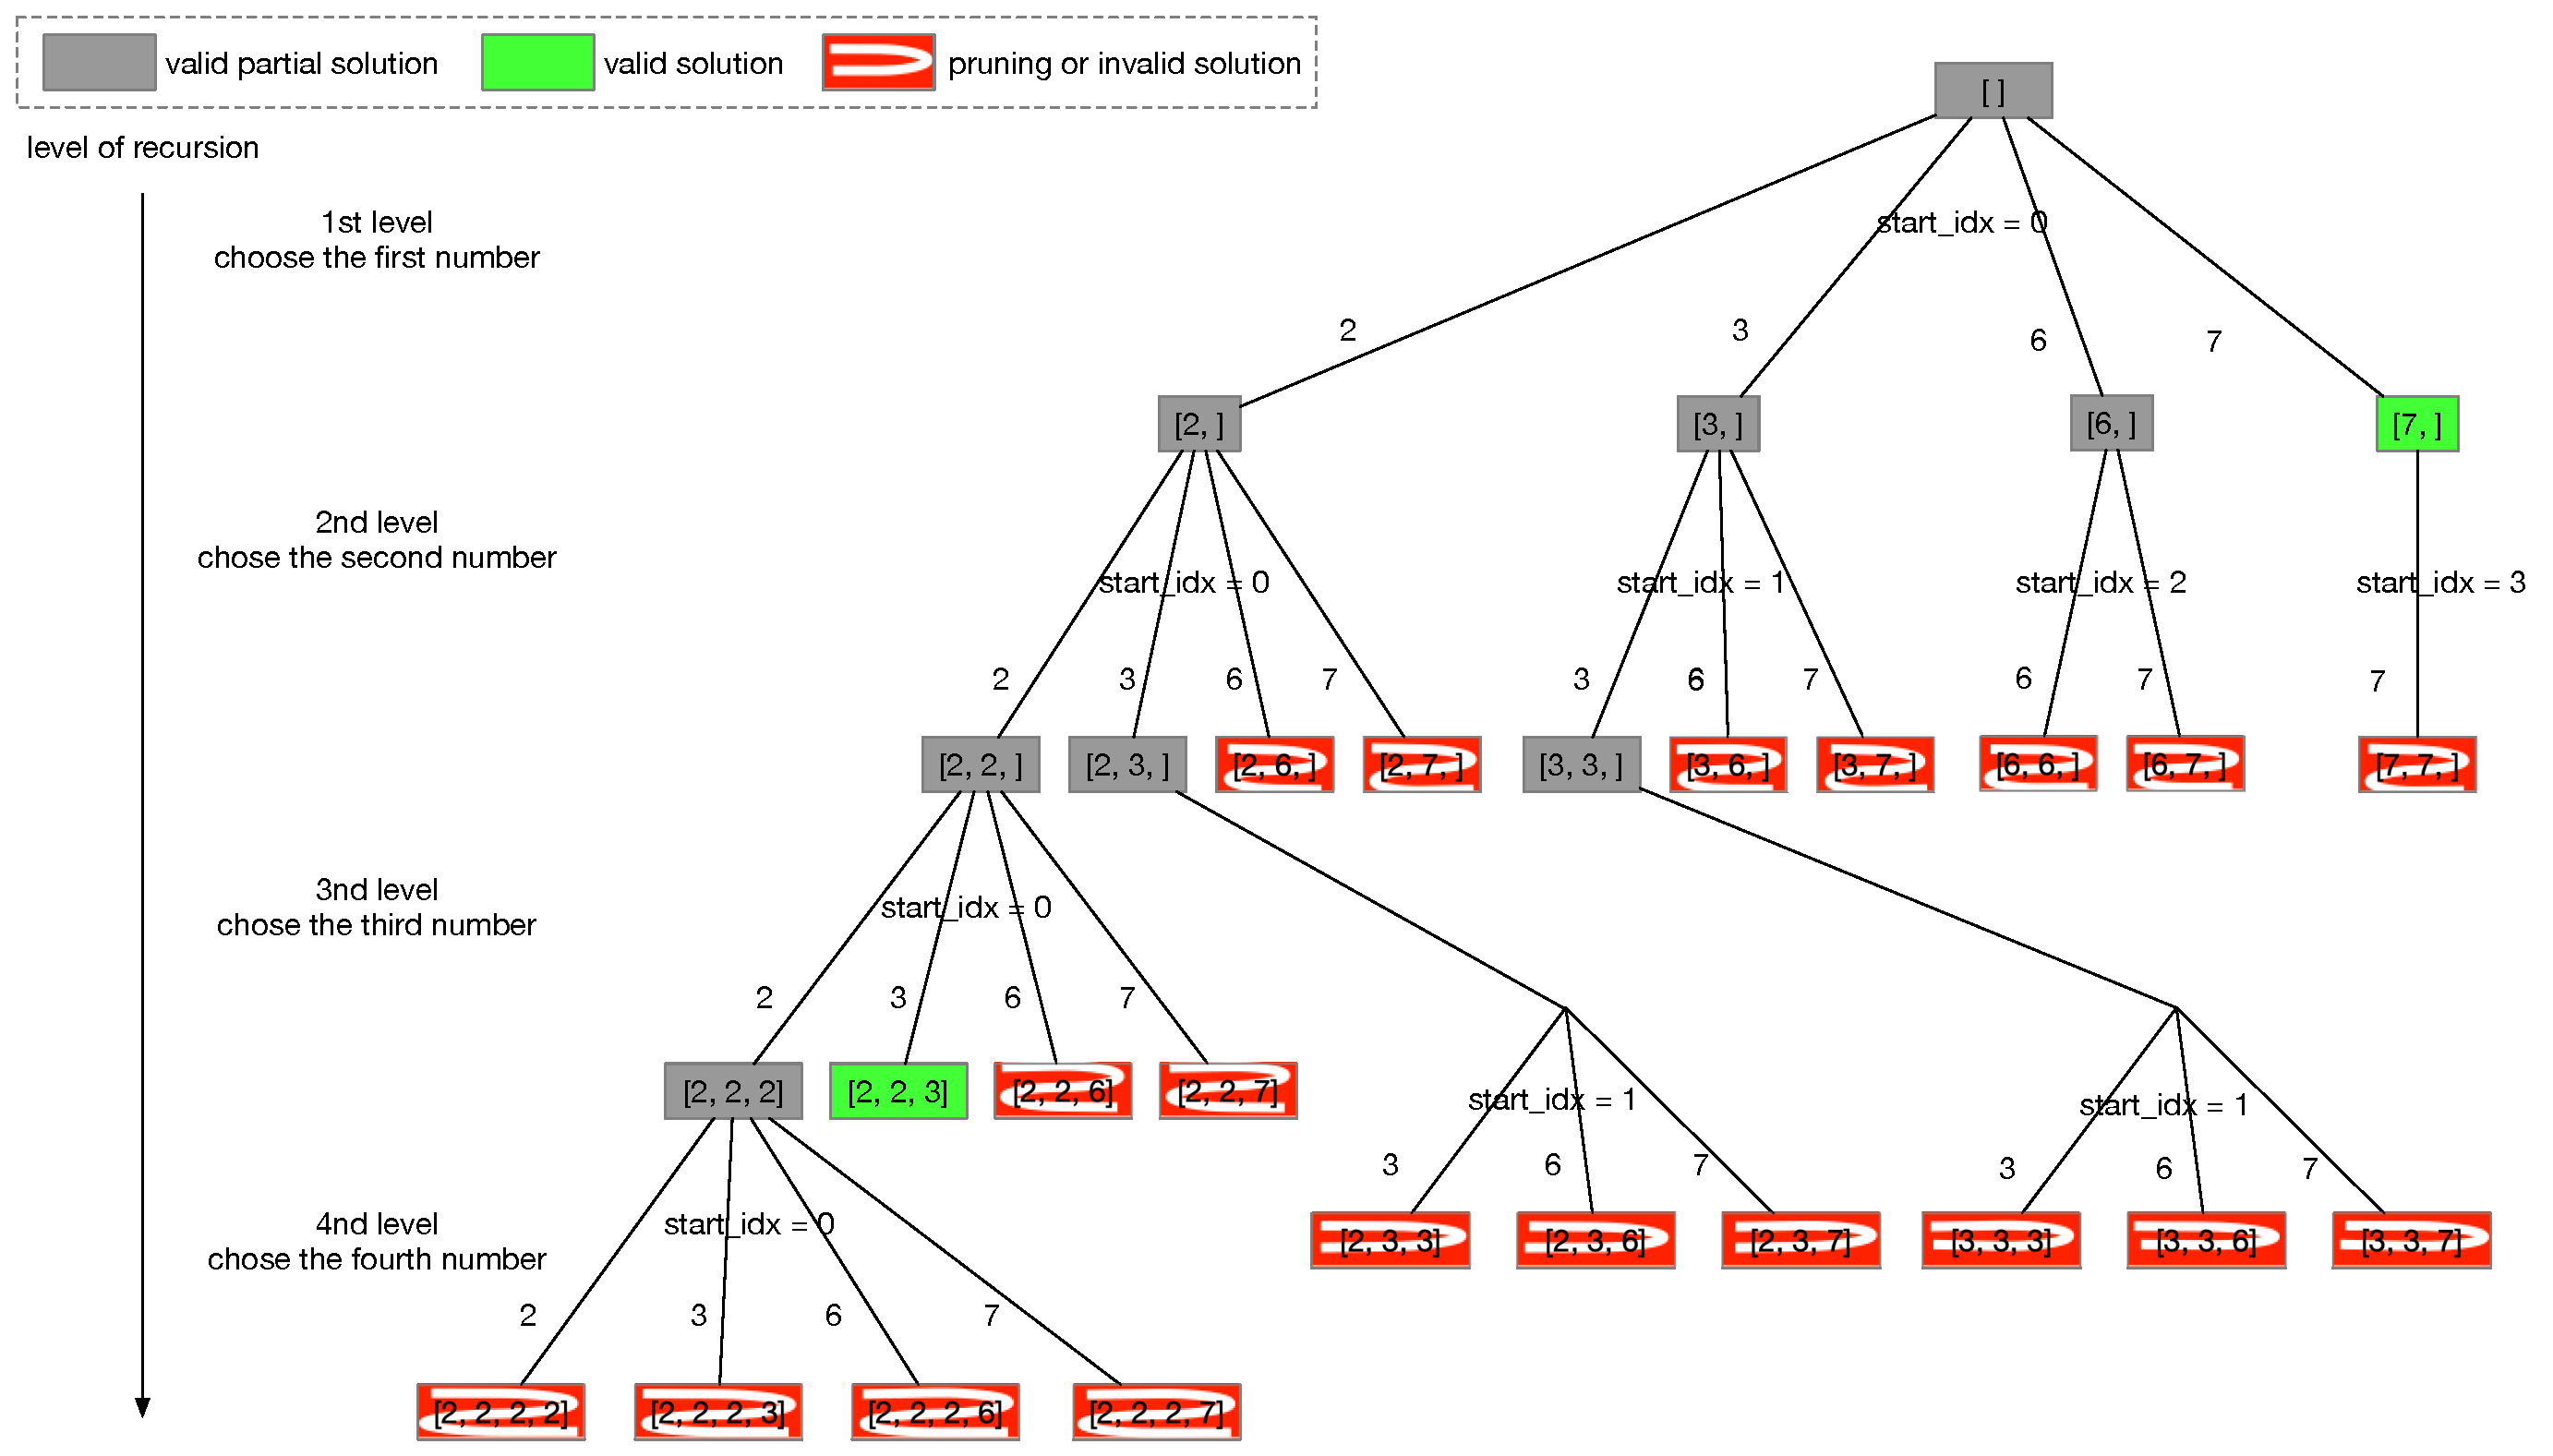
\includegraphics[width=1.0\linewidth]{images/lc0039_pst}
	\label{fig:lc0039pst}
\end{figure}

\subsection*{Solution 2 - Backtracking (with more pruning)}
\begin{lstlisting}
std::vector<std::vector<int>> combinationSum(std::vector<int>& candidates, int target) {
	std::vector<std::vector<int>> solutions;
	std::vector<int> comb;
	std::sort(candidates.begin(), candidates.end());
	Backtracking(candidates, target, 0, comb, solutions);
	return solutions;
}

void Backtracking(const std::vector<int>& candidates, int target, int start, 
								  std::vector<int>& comb, std::vector<std::vector<int>>& solutions) {
	// valid solution (base case)
	if (target == 0) {
		solutions.push_back(comb);
		return;
	}
	for (int i = start; i < candidates.size(); ++i) {
		// pruning
		if (candidates[i] > target) { break; }
		comb.push_back(candidates[i]);
		Backtracking(candidates, target - candidates[i], i, comb, solutions);
		comb.pop_back();
	}
}
\end{lstlisting}\mbox{}

In the case of {\colorbox{CodeBackground}{\lstinline|candidates = [2, 3 ,6, 7]|}} and {\colorbox{CodeBackground}{\lstinline|target = 7|}}, the {\color{blue}{potential search tree}} is as follows. \\

It should be noted that the {\color{blue}{search order}} is implicitly set to ensure that each potential solution is visited exactly once.

\begin{figure}[H]
	\centering
	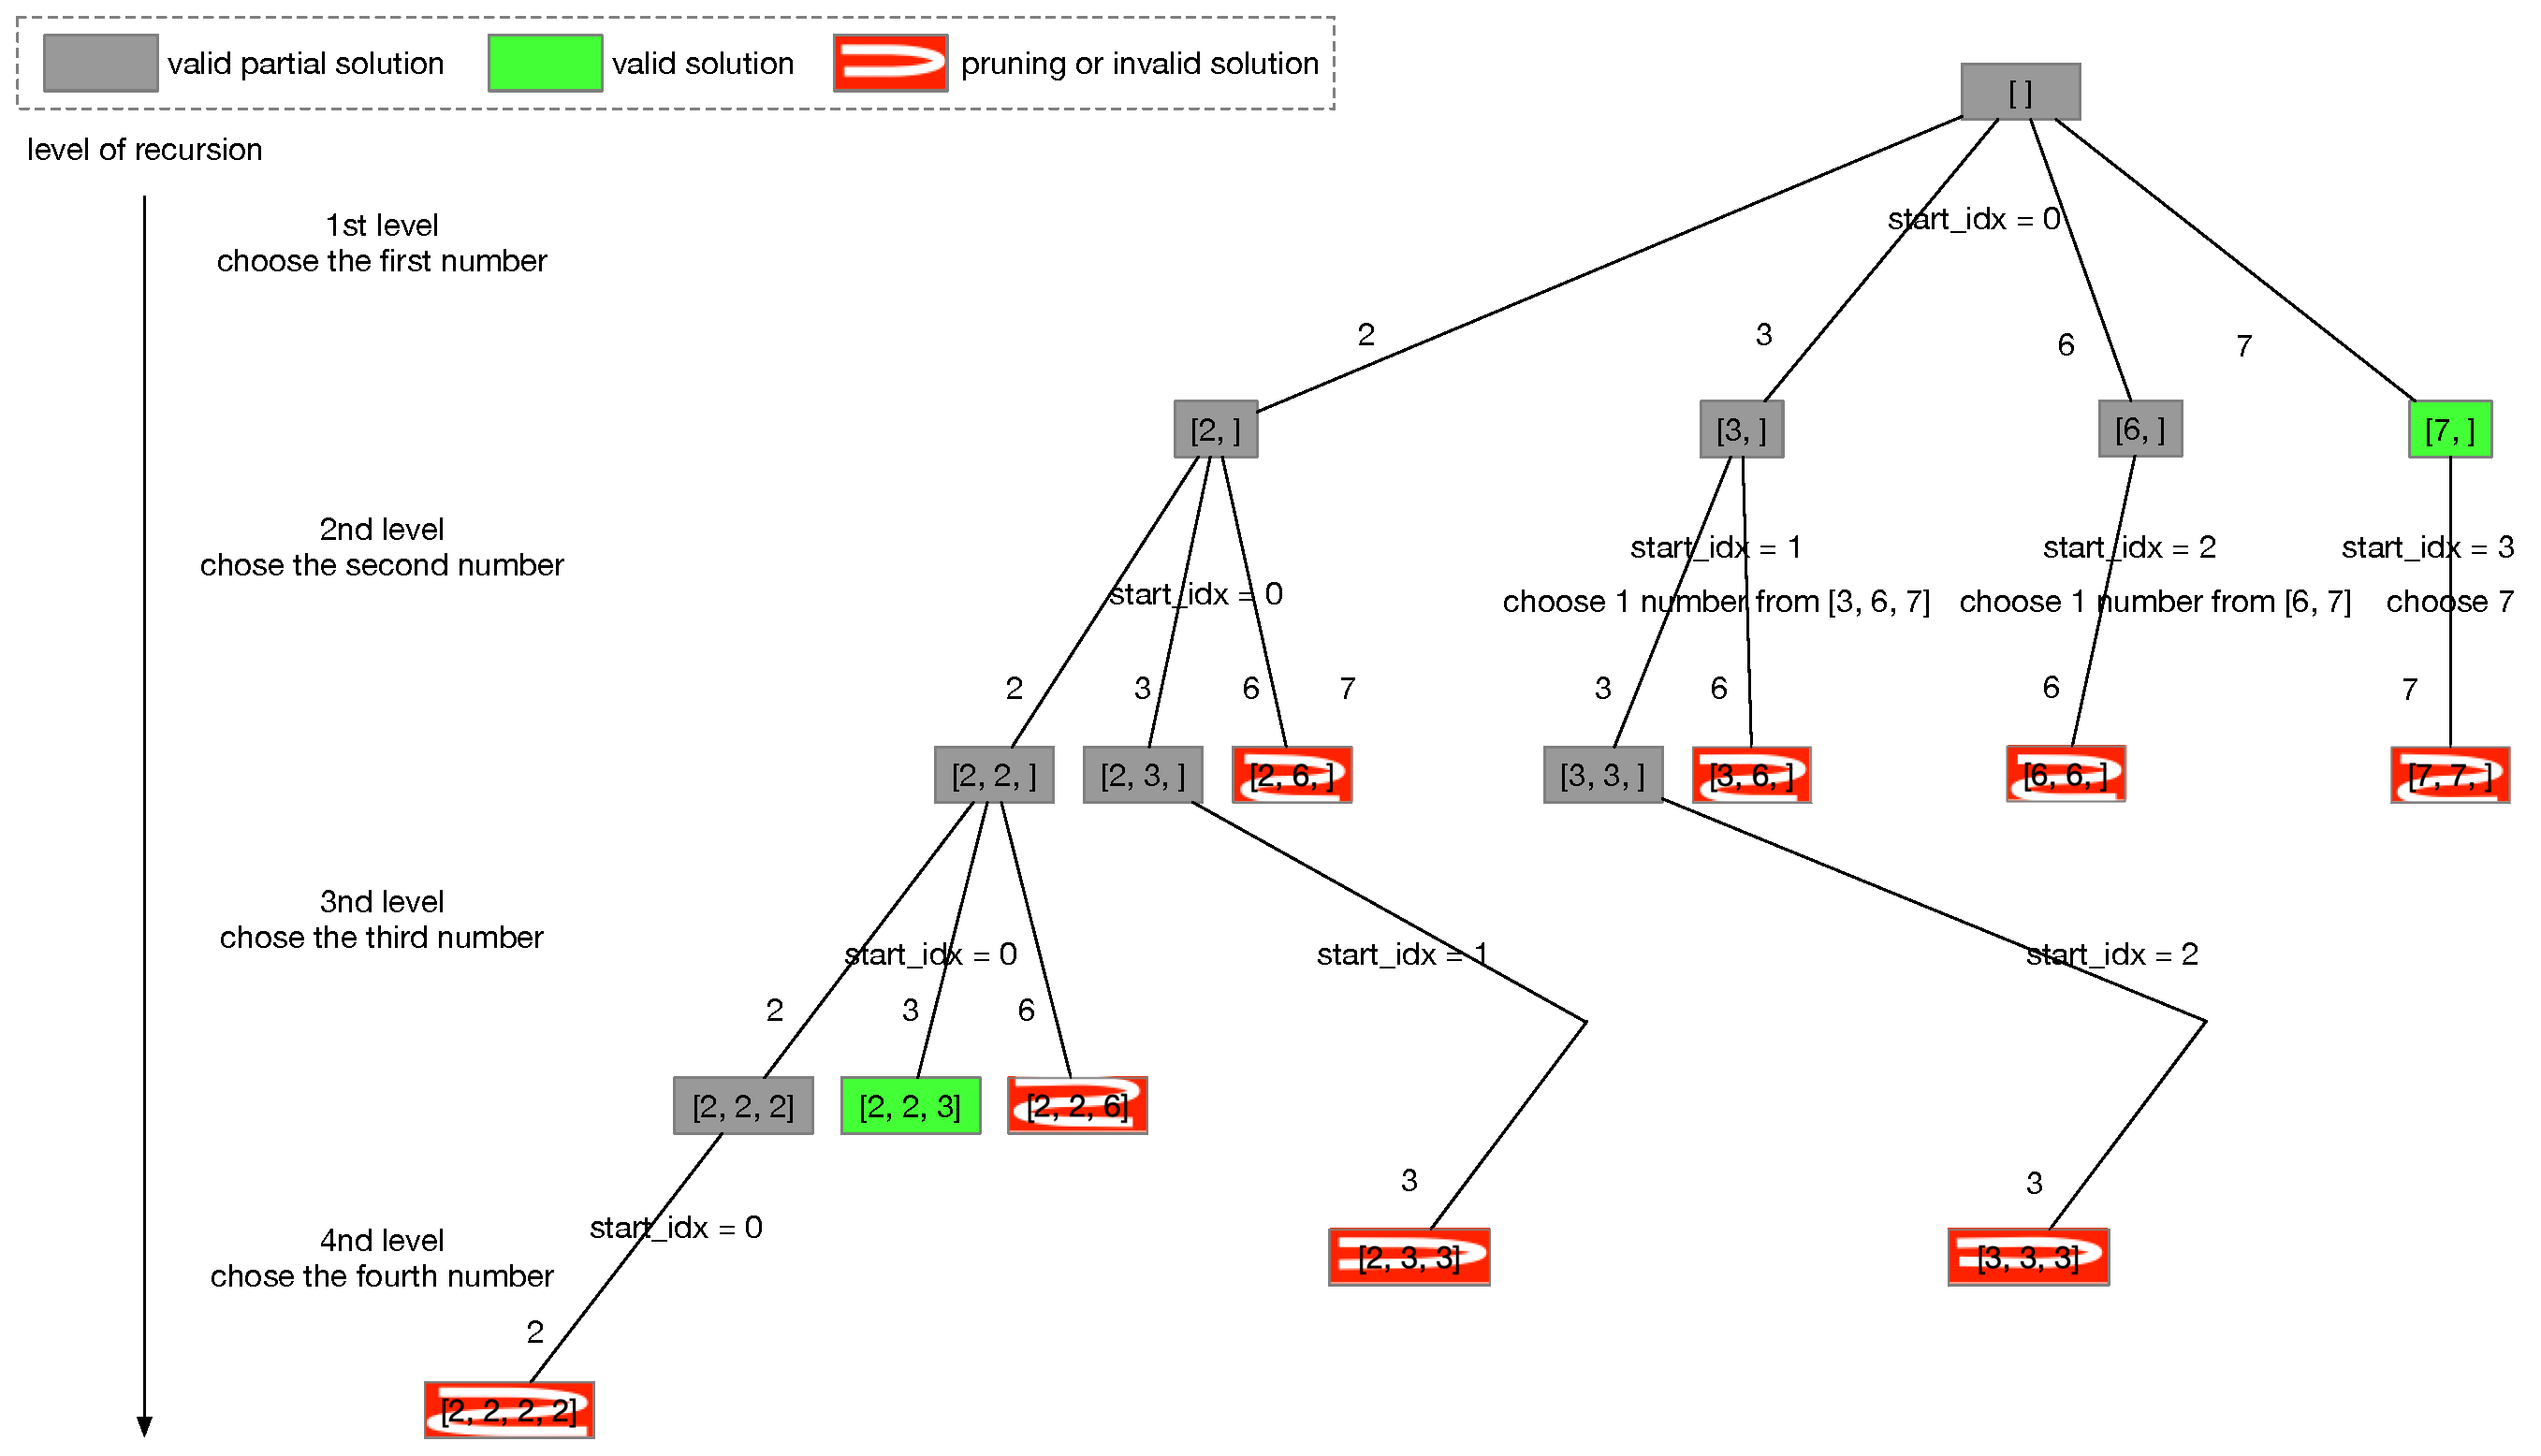
\includegraphics[width=1.0\linewidth]{images/lc0039_pst_2}
	\label{fig:lc0039pst2}
\end{figure}

\subsection*{Related}
\begin{itemize}
	\item \hyperref[lc0039]{LC 0039 - Combination Sum}
	\item \hyperref[lc0040]{LC 0040 - Combination Sum II}
	\item \hyperref[lc0216]{LC0216 - Combination Sum III}
%	\item \hyperref[lc0377]{LC 0377 - Combination Sum IV}
\end{itemize}

\section{LC 0040 - Combination Sum II}\label{lc0040}
Given a \ul{non-empty} \ul{array} of \ul{integers} {\colorbox{CodeBackground}{\lstinline|candidates|}} (which may contain duplicates) ({\colorbox{CodeBackground}{\lstinline|candidates[i] >= 1|}}) and a \ul{target integer} {\colorbox{CodeBackground}{\lstinline|target|}} ({\colorbox{CodeBackground}{\lstinline|target >= 1|}}), return a list of all \ul{combinations} of integers in {\colorbox{CodeBackground}{\lstinline|candidates|}} that add up to {\colorbox{CodeBackground}{\lstinline|target|}}.\\

Each number in {\colorbox{CodeBackground}{\lstinline|candidates|}} may be used \ul{only once} in the combination.\\

You may return the combinations in any order.\\

Examples:
\begin{itemize}
	\item {\colorbox{CodeBackground}{\lstinline|candidates = [10,1,2,7,6,1,5], target = 8 --> [[1,1,6], [1,2,5], [1,7], [2,6]]|}}
	\item {\colorbox{CodeBackground}{\lstinline|candidates = [2,5,2,1,2], target = 5 --> [[1,2,2], [5]]|}}
\end{itemize}

\subsection*{Solution - Backtracking}
\begin{lstlisting}
std::vector<std::vector<int>> combinationSum2(std::vector<int>& candidates, int target) {
	std::vector<std::vector<int>> solutions;
	std::vector<int> comb;
	std::sort(candidates.begin(), candidates.end());
	Backtracking(candidates, target, 0, comb, solutions);
	return solutions;
}

void Backtracking(const std::vector<int>& candidates, int target, int start, 
								  std::vector<int>& comb, std::vector<std::vector<int>>& solutions) {
	// valid solution (base case)
	if (target == 0) {
		solutions.push_back(comb);
		return;
	}
	for (int i = start; i < candidates.size(); ++i) {
		// pruning (skip duplicates)
		if (i > start && candidates[i] == candidates[i - 1]) { continue; }
		// pruning
		if (candidates[i] > target) { break; }
		comb.push_back(candidates[i]);
		Backtracking(candidates, target - candidates[i], i + 1, comb, solutions);
		comb.pop_back();
	}
}
\end{lstlisting}

\subsection*{Related}
\begin{itemize}
	\item \hyperref[lc0039]{LC 0039 - Combination Sum}
	\item \hyperref[lc0040]{LC 0040 - Combination Sum II}
	\item \hyperref[lc0216]{LC0216 - Combination Sum III}
%	\item \hyperref[lc0377]{LC 0377 - Combination Sum IV}
\end{itemize}

\section{LC 0216 - Combination Sum III}\label{lc0216}
Find all valid \ul{combinations} of {\colorbox{CodeBackground}{\lstinline|k|}} \ul{distinct numbers} that sum up to {\colorbox{CodeBackground}{\lstinline|target|}} such that the following conditions are true:
\begin{itemize}
	\item Only numbers {\colorbox{CodeBackground}{\lstinline|1|}} to {\colorbox{CodeBackground}{\lstinline|9|}} are used.
	\item Each number is used \ul{only once}.
\end{itemize}

Return a list of all possible valid combinations.\\

Note that:
\begin{itemize}
	\item {\colorbox{CodeBackground}{\lstinline|2 <= k <= 9|}} and {\colorbox{CodeBackground}{\lstinline|1 <= target <= 60|}}.
	\item You may return the combinations in any order.
\end{itemize}

Examples:
\begin{itemize}
	\item {\colorbox{CodeBackground}{\lstinline|k = 3, target = 7 --> [[1,2,4]]|}}
	\item {\colorbox{CodeBackground}{\lstinline|k = 3, target = 9 --> [[1,2,6],[1,3,5],[2,3,4]]|}}
	\item {\colorbox{CodeBackground}{\lstinline|k = 4, target = 1 --> []|}}
\end{itemize}

\subsection*{Solution - Backtracking}
\begin{lstlisting}
std::vector<std::vector<int>> combinationSum3(int k, int target) {
	std::vector<std::vector<int>> solutions;
	std::vector<int> comb;
	Backtracking(k, target, 1, comb, solutions);
	return solutions;
}

void Backtracking(int k, int target, int start, std::vector<int>& comb,
std::vector<std::vector<int>>& solutions) {
	// valid solution (base case)
	if (k == 0 && target == 0) {
		solutions.push_back(comb);
		return;
	}
	for (int i = start; i <= 9; ++i) {
		// pruning
		if (i > target) { break; }
		comb.push_back(i);
		Backtracking(k - 1, target - i, i + 1, comb, solutions);
		comb.pop_back();
	}
}
\end{lstlisting}\mbox{}

In the case of {\colorbox{CodeBackground}{\lstinline|k=3|}} and {\colorbox{CodeBackground}{\lstinline|target = 7|}}, the {\color{blue}{potential search tree}} is as follows. \\

It should be noted that the {\color{blue}{search order}} is implicitly set to ensure that each potential solution is visited exactly once.

\begin{figure}[H]
	\centering
	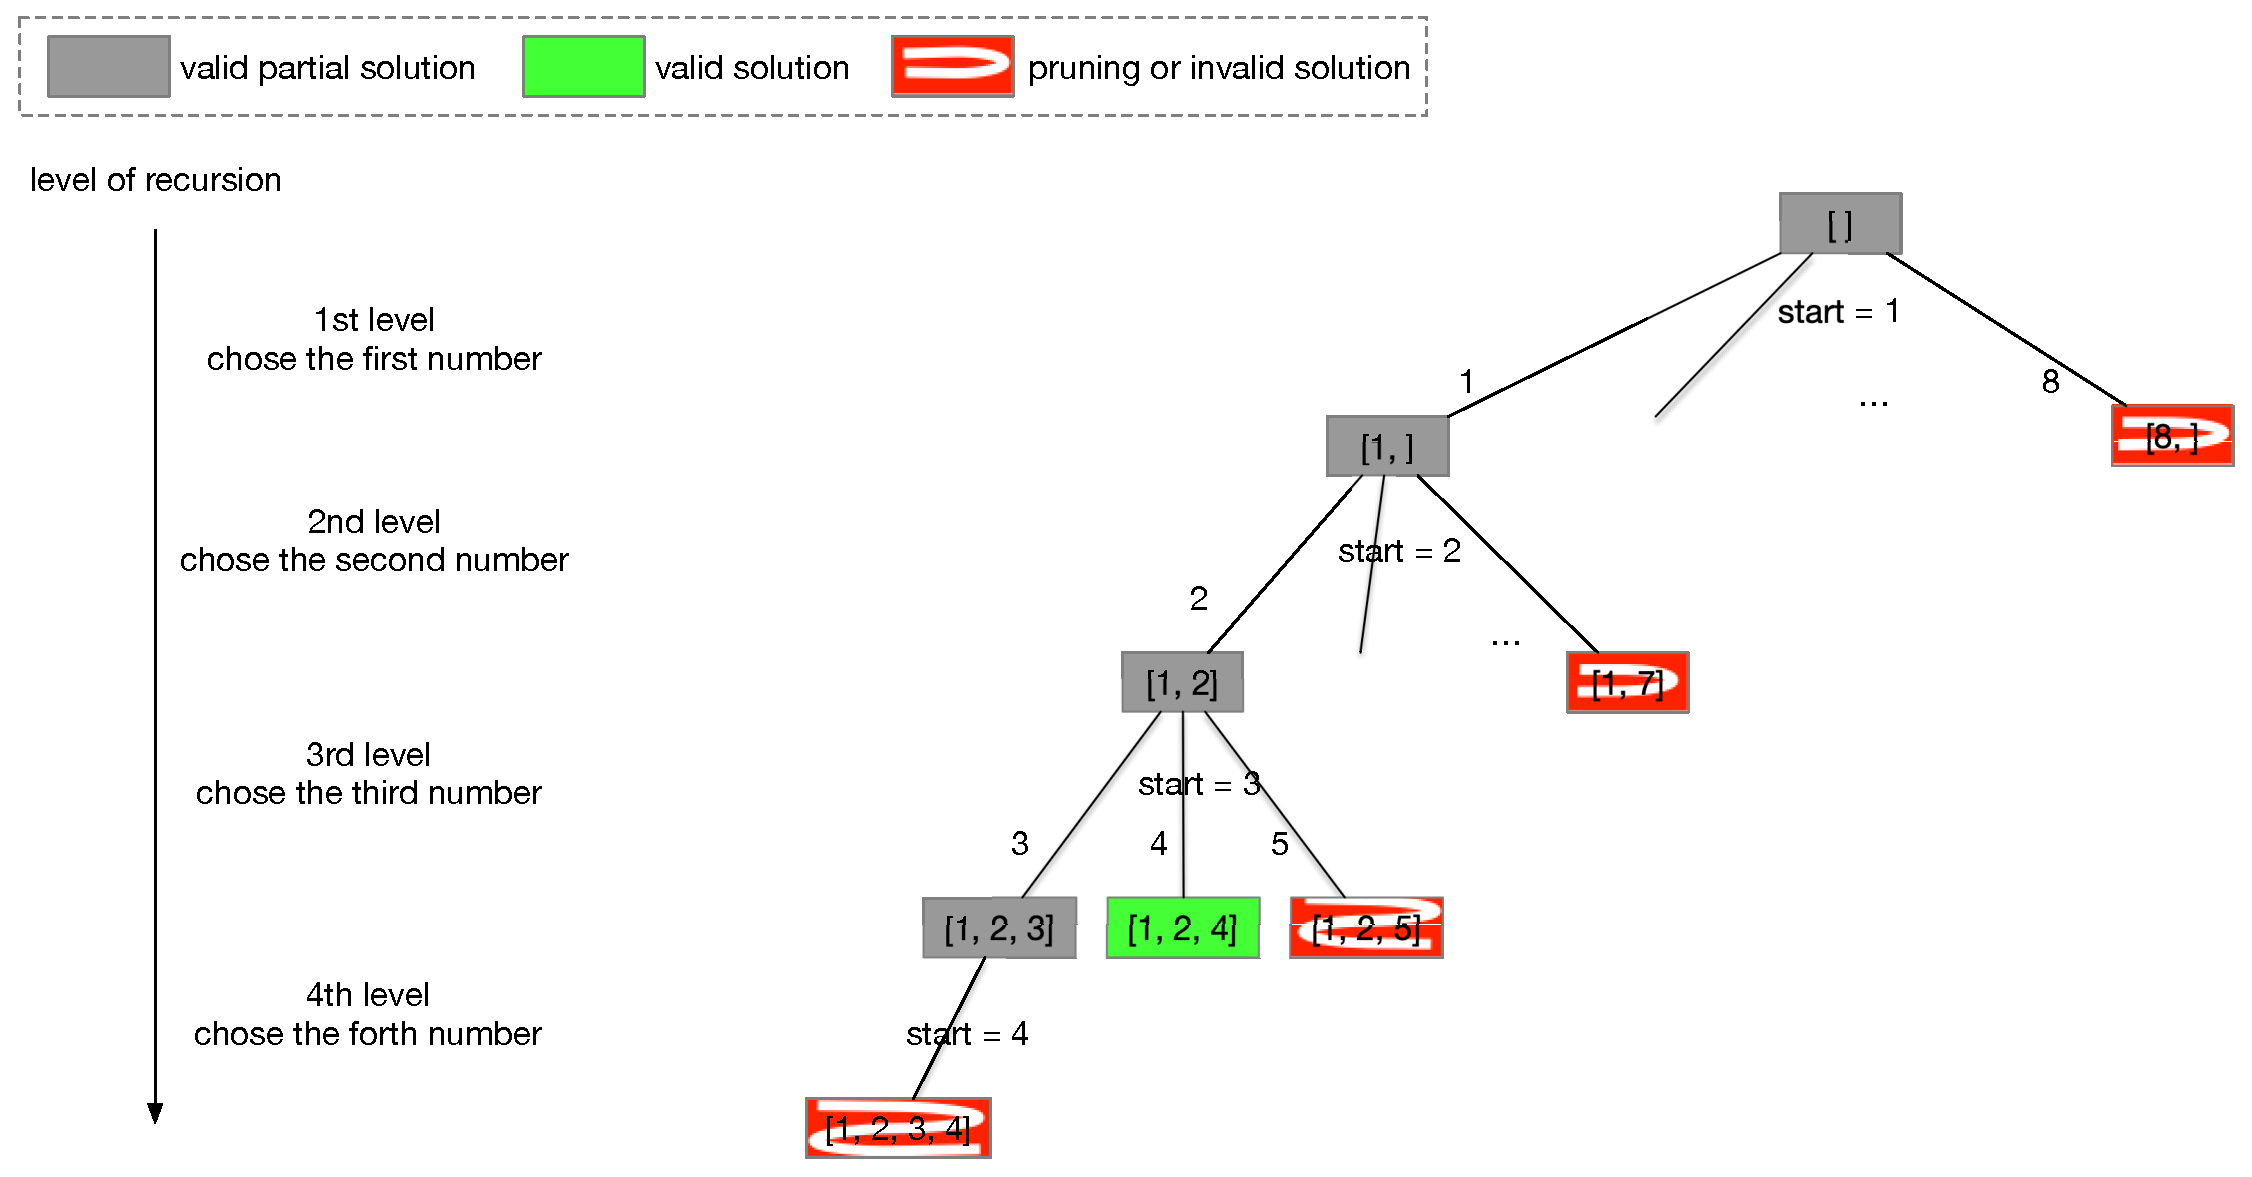
\includegraphics[width=1.0\linewidth]{images/lc0216_pst}
	\label{fig:lc0216pst}
\end{figure}

\subsection*{Related}
\begin{itemize}
	\item \hyperref[lc0039]{LC 0039 - Combination Sum}
	\item \hyperref[lc0040]{LC 0040 - Combination Sum II}
	\item \hyperref[lc0216]{LC0216 - Combination Sum III}
%	\item \hyperref[lc0377]{LC 0377 - Combination Sum IV}
\end{itemize}

\section{LC 0022 - Generate Parentheses}
Given {\colorbox{CodeBackground}{\lstinline|n|}} ({\colorbox{CodeBackground}{\lstinline|n >= 1|}}) pairs of parentheses, write a function to generate all \ul{combinations} of well-formed parentheses.\\

Examples:
\begin{itemize}
	\item {\colorbox{CodeBackground}{\lstinline|n = 3 --> ["((()))","(()())","(())()","()(())","()()()"]|}}
	\item {\colorbox{CodeBackground}{\lstinline|n = 1 --> ["()"]|}}
\end{itemize}

\subsection*{Solution - Backtracking}
\begin{lstlisting}
std::vector<std::string> generateParenthesis(int n) {
  std::vector<std::string> solutions;
  std::string comb;
  Backtracking(n, 0, 0, comb, solutions);
  return solutions;
}

void Backtracking(int n, int open, int close, std::string& comb,
                  std::vector<std::string>& solutions) {
  // valid solution (base case)
  if (comb.size() == n * 2) {
    solutions.push_back(comb);
    return;
  }
  if (open < n) {
    comb.push_back('(');
    Backtracking(n, open + 1, close, comb, solutions);
    comb.pop_back();
  }
  if (close < open) {
    comb.push_back(')');
    Backtracking(n, open, close + 1, comb, solutions);
    comb.pop_back();
  }
}
\end{lstlisting}

\section{LC 0046 - Permutations}
Given a \ul{non-empty} array {\colorbox{CodeBackground}{\lstinline|nums|}} of \ul{distinct integers}, return all the \ul{permutations} of {\colorbox{CodeBackground}{\lstinline|nums|}}. \\

You may return the permutations in any order.\\

Examples:
\begin{itemize}
	\item {\colorbox{CodeBackground}{\lstinline|nums = [1,2,3] --> [[1,2,3],[1,3,2],[2,1,3],[2,3,1],[3,1,2],[3,2,1]]|}}
	\item {\colorbox{CodeBackground}{\lstinline|nums = [0,1] --> [[0,1],[1,0]]|}}
	\item {\colorbox{CodeBackground}{\lstinline|nums = [1] --> [[1]]|}}
\end{itemize}

\subsection*{Solution - Backtracking}
\begin{lstlisting}
std::vector<std::vector<int>> permute(const std::vector<int>& nums) {
	std::vector<std::vector<int>> solutions;
	std::vector<int> perm;
	std::vector<bool> used(nums.size(), false);
	Backtracking(nums, used, perm, solutions);
	return solutions;
}

void Backtracking(const std::vector<int>& nums, std::vector<bool>& used, 
								  std::vector<int>& perm, std::vector<std::vector<int>>& solutions) {
	// valid solution (base case)
	if (perm.size() == nums.size()) {
		solutions.push_back(perm);
		return;
	}
	for (int i = 0; i < nums.size(); ++i) {
		// pruning
		if (used[i]) { continue; }
		used[i] = true;
		perm.push_back(nums[i]);
		Backtracking(nums, used, perm, solutions);
		used[i] = false;
		perm.pop_back();
	}
}
\end{lstlisting}

\section{LC 0047 - Permutations II}
Given a \ul{non-empty} array {\colorbox{CodeBackground}{\lstinline|nums|}} which \ul{might contain duplicates}, return all permutations of {\colorbox{CodeBackground}{\lstinline|nums|}}.\\

You may return the permutations in any order.\\

Examples:
\begin{itemize}
	\item {\colorbox{CodeBackground}{\lstinline|nums = [1,1,2] --> [[1,1,2], [1,2,1], [2,1,1]]|}}
	\item {\colorbox{CodeBackground}{\lstinline|nums = [1,2,3] --> [[1,2,3],[1,3,2],[2,1,3],[2,3,1],[3,1,2],[3,2,1]]|}}
\end{itemize}

\subsection*{Solution - Backtracking}
\begin{lstlisting}
std::vector<std::vector<int>> permuteUnique(std::vector<int>& nums) {
  std::sort(nums.begin(), nums.end());
  std::vector<std::vector<int>> solutions;
  std::vector<int> perm;
  std::vector<bool> used(nums.size(), false);
  Backtracking(nums, used, perm, solutions);
  return solutions;
}

void Backtracking(const std::vector<int>& nums, std::vector<bool>& used,
                  std::vector<int>& perm, std::vector<std::vector<int>>& solutions) {
  // valid solution (base case)
  if (perm.size() == nums.size()) {
    solutions.push_back(perm);
    return;
  }
  for (int i = 0; i < nums.size(); ++i) {
    // pruning
    if (used[i] || (i > 0 && nums[i] == nums[i - 1] && !used[i - 1])) { continue; }
    used[i] = true;
    perm.push_back(nums[i]);
    Backtracking(nums, used, perm, solutions);
    used[i] = false;
    perm.pop_back();
  }
}
\end{lstlisting}

\section{LC 0078 - Subsets}
Given a \ul{non-empty} array {\colorbox{CodeBackground}{\lstinline|nums|}} of \ul{distinct integers}, return all subsets (power set) of {\colorbox{CodeBackground}{\lstinline|nums|}}.\\

You may return the subsets in any order.\\

Examples:
\begin{itemize}
	\item {\colorbox{CodeBackground}{\lstinline|nums = [1,2,3] --> [[],[1],[2],[1,2],[3],[1,3],[2,3],[1,2,3]]|}}
	\item {\colorbox{CodeBackground}{\lstinline|nums = [0] --> [[],[0]]|}}
\end{itemize}

\subsection*{Solution - Backtracking}
\begin{lstlisting}
std::vector<std::vector<int>> subsets(std::vector<int>& nums) {
	std::vector<std::vector<int>> solutions;
	std::vector<int> subset;
	Backtracking(nums, 0, subset, solutions);
	return solutions;
}

void Backtracking(std::vector<int>& nums, int start, std::vector<int>& subset,
								  std::vector<std::vector<int>>& solutions) {
	// // valid solution (base case)
	solutions.push_back(subset);
	for (int i = start; i < nums.size(); i++) {
		subset.push_back(nums[i]);
		Backtracking(nums, i + 1, subset, solutions);
		subset.pop_back();
	}
}
\end{lstlisting}

\section{LC 0090 - Subsets II}
Given a \ul{non-empty} array {\colorbox{CodeBackground}{\lstinline|nums|}} which \ul{might contain duplicates}, return all subsets (power set) of {\colorbox{CodeBackground}{\lstinline|nums|}}.\\

You may return the subsets in any order.\\

Examples:
\begin{itemize}
	\item {\colorbox{CodeBackground}{\lstinline|nums = [1,2,2] --> [[],[1],[1,2],[1,2,2],[2],[2,2]]|}}
	\item {\colorbox{CodeBackground}{\lstinline|nums = [0] --> [[],[0]]|}}
\end{itemize}

\subsection*{Solution - Backtracking}
\begin{lstlisting}
std::vector<std::vector<int>> subsetsWithDup(std::vector<int>& nums) {
	std::sort(nums.begin(), nums.end());
	std::vector<std::vector<int>> solutions;
	std::vector<int> subset;
	Backtracking(nums, 0, subset, solutions);
	return solutions;
}

void Backtracking(const std::vector<int>& nums, int index, std::vector<int>& subset,
								  std::vector<std::vector<int>>& solutions) {
	// valid solution (base case)
	solutions.push_back(subset);
	for (int i = index; i < nums.size(); ++i) {
		// pruning
		if (i > index && nums[i] == nums[i - 1]) { continue; }
		subset.push_back(nums[i]);
		Backtracking(nums, i + 1, subset, solutions);
		subset.pop_back();
	}
}
\end{lstlisting}

\section{LC 0131 - Palindrome Partitioning}
Given a \ul{non-empty} string {\colorbox{CodeBackground}{\lstinline|s|}}, partition {\colorbox{CodeBackground}{\lstinline|s|}} such that every substring of the partition is a \ul{palindrome}. Return all palindrome partitioning of {\colorbox{CodeBackground}{\lstinline|s|}}.\\

Examples:
\begin{itemize}
	\item {\colorbox{CodeBackground}{\lstinline|s = "aab" --> [["a","a","b"],["aa","b"]]|}}
	\item {\colorbox{CodeBackground}{\lstinline|s = "a" --> [["a"]]|}}
\end{itemize}

\subsection*{Solution - Backtracking}
\begin{lstlisting}
std::vector<std::vector<std::string>> partition(std::string s) {
	std::vector<std::vector<std::string>> solutions;
	std::vector<std::string> part;
	Backtracking(s, 0, part, solutions);
	return solutions;
}

bool isPalindrome(const std::string& s, int start, int end) {
	while (start < end) {
		if (s[start++] != s[end--]) { return false; }
	}
	return true;
}

void Backtracking(const std::string& s, int idx, std::vector<std::string>& part,
std::vector<std::vector<std::string>>& solutions) {
	// valid solution (base case)
	if (idx == s.size()) {
		solutions.push_back(part);
		return;
	}
	for (int i = idx; i < s.size(); i++) {
		if (isPalindrome(s, idx, i)) {
			part.push_back(s.substr(idx, i - idx + 1));
			Backtracking(s, i + 1, part, solutions);
			part.pop_back();
		}
	}
}
\end{lstlisting}

\section{LC 0093 - Restore IP Addresses}
A valid IP address consists of exactly four integers separated by single dots. Each integer is between {\colorbox{CodeBackground}{\lstinline|0|}} and {\colorbox{CodeBackground}{\lstinline|255|}} and cannot have leading zeros.\\

For example, {\colorbox{CodeBackground}{\lstinline|"0.1.2.201"|}} and {\colorbox{CodeBackground}{\lstinline|"192.168.1.1"|}} are valid IP addresses, but {\colorbox{CodeBackground}{\lstinline|"0.011.255.245"|}}, {\colorbox{CodeBackground}{\lstinline|"192.168.1.312"|}} and {\colorbox{CodeBackground}{\lstinline|"192.168@1.1"|}} are invalid IP addresses.\\

Given a \ul{non-empty} string {\colorbox{CodeBackground}{\lstinline|s|}} containing only digits, return all valid IP addresses that can be formed by \ul{inserting dots} into {\colorbox{CodeBackground}{\lstinline|s|}}.\\

You may return the valid IP addresses in any order. \\

Examples:
\begin{itemize}
	\item {\colorbox{CodeBackground}{\lstinline|s = "25525511135" --> ["255.255.11.135","255.255.111.35"]|}}
	\item {\colorbox{CodeBackground}{\lstinline|s = "0000" --> ["0.0.0.0"]|}}
	\item {\colorbox{CodeBackground}{\lstinline|s = "101023" --> ["1.0.10.23","1.0.102.3","10.1.0.23","10.10.2.3","101.0.2.3"]|}}
\end{itemize}

\subsection*{Solution - Backtracking}
\begin{lstlisting}
std::vector<std::string> restoreIpAddresses(std::string s) {
	std::vector<std::string> solutions;
	std::string ip;
	Backtracking(s, 0, 0, ip, solutions);
	return solutions;
}

void Backtracking(const std::string& s, int start, int num_part, std::string& ip,
								  std::vector<std::string>& solutions) {
	// valid solution (base case)
	if (num_part == 4 && start == s.size()) { solutions.push_back(ip); }
	
	// pruning
	if (num_part >= 4) { return; }
	
	for (int len = 1; len <= 3; ++len) {
		// pruning
		if (start + len > s.size()) { break; }
		
		// get the current part
		std::string part = s.substr(start, len);
		
		// pruning
		if ((part[0] == '0' && part.size() > 1) || (len == 3 && std::stoi(part) > 255)) { continue; }
		
		ip += part;
		if (num_part < 3) ip += '.';
		Backtracking(s, start + len, num_part + 1, ip, solutions);
		ip.erase(ip.end() - len, ip.end());
		if (num_part < 3) ip.pop_back();
	}
}

\end{lstlisting}

\section{LC 0079 - Word Search}
Given an {\colorbox{CodeBackground}{\lstinline|m x n|}} ({\colorbox{CodeBackground}{\lstinline|m, n >= 1|}}) grid of characters {\colorbox{CodeBackground}{\lstinline|board|}} and a string {\colorbox{CodeBackground}{\lstinline|word|}}, return {\colorbox{CodeBackground}{\lstinline|true|}} if {\colorbox{CodeBackground}{\lstinline|word|}} exists in the grid.\\

The word can be constructed from letters of sequentially adjacent cells, where adjacent cells are horizontally or vertically neighboring. The same letter cell may not be used more than once.\\

Examples:
\begin{itemize}
	\item {\colorbox{CodeBackground}{\lstinline|board = [["A","B","C","E"],["S","F","C","S"],["A","D","E","E"]], word = "ABCCED" --> true|}}
	\begin{figure}[H]
		\centering
		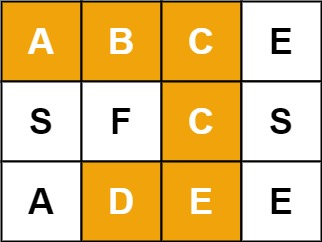
\includegraphics[width=0.2\linewidth]{images/lc0079_example1}
		\label{fig:lc0079example1}
	\end{figure}
	\item {\colorbox{CodeBackground}{\lstinline|board = [["A","B","C","E"],["S","F","C","S"],["A","D","E","E"]], word = "SEE" --> true|}}
	\begin{figure}[H]
		\centering
		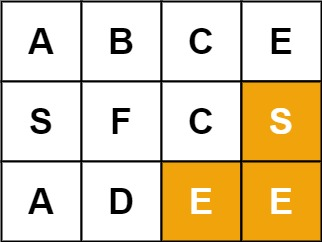
\includegraphics[width=0.2\linewidth]{images/lc0079_example2}
		\label{fig:lc0079example2}
	\end{figure}
	\item {\colorbox{CodeBackground}{\lstinline|board = [["A","B","C","E"],["S","F","C","S"],["A","D","E","E"]], word = "ABCB" --> false|}}
	\begin{figure}[H]
		\centering
		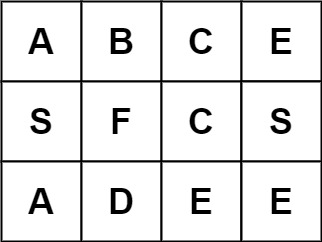
\includegraphics[width=0.2\linewidth]{images/lc0079_example3}
		\label{fig:lc0079example3}
	\end{figure}
\end{itemize}

\subsection*{Solution - Backtracking}

\section{LC 0052 - N-Queens II}
The {\colorbox{CodeBackground}{\lstinline|n|}}-queens problem is to place {\colorbox{CodeBackground}{\lstinline|n|}} queens on an {\colorbox{CodeBackground}{\lstinline|n x n|}} chessboard such that no two queens attack each other.\\

Given an integer {\colorbox{CodeBackground}{\lstinline|n|}}, return the number of distinct solutions to the {\colorbox{CodeBackground}{\lstinline|n|}}-queens problem.\\

Example: {\colorbox{CodeBackground}{\lstinline|n = 4 --> 2|}}
\begin{figure}[H]
	\centering
	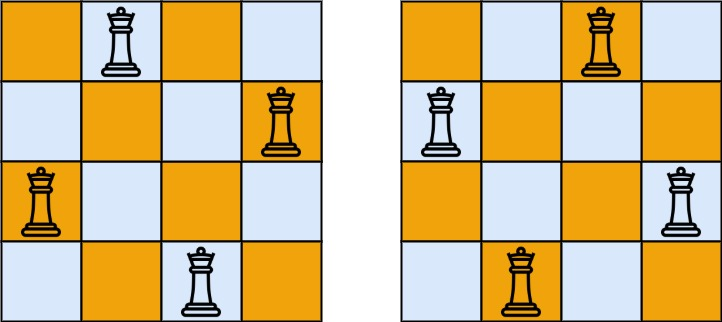
\includegraphics[width=0.45\linewidth]{images/lc0051_example}
	\label{fig:lc0052example}
\end{figure}

\subsection*{Solution - Backtracking}

\section{LC 0051 - N-Queens}
The {\colorbox{CodeBackground}{\lstinline|n|}}-queens problem is to place {\colorbox{CodeBackground}{\lstinline|n|}} queens on an {\colorbox{CodeBackground}{\lstinline|n x n|}} chessboard such that no two queens attack each other.\\

Given an integer {\colorbox{CodeBackground}{\lstinline|n|}}, return all distinct solutions to the {\colorbox{CodeBackground}{\lstinline|n|}}-queens problem. Each solution contains a distinct board configuration of the {\colorbox{CodeBackground}{\lstinline|n|}}-queens' placement, where {\colorbox{CodeBackground}{\lstinline|'Q'|}} and {\colorbox{CodeBackground}{\lstinline|'.'|}} both indicate a queen and an empty space, respectively.\\

You may return the answer in any order.\\

Example: {\colorbox{CodeBackground}{\lstinline|n = 4 --> [[".Q..","...Q","Q...","..Q."],["..Q.","Q...","...Q",".Q.."]]|}}
\begin{figure}[H]
	\centering
	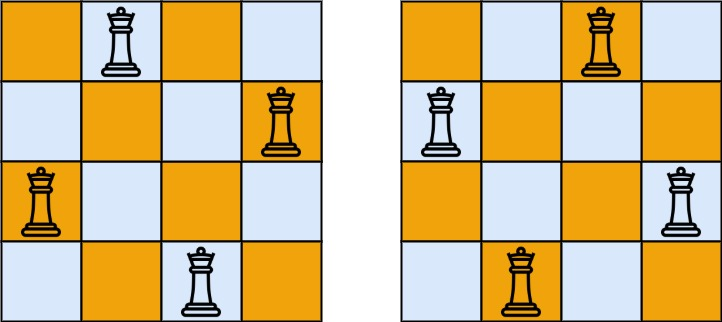
\includegraphics[width=0.45\linewidth]{images/lc0051_example}
	\label{fig:lc0051example}
\end{figure}

\subsection*{Solution - Backtracking}

\section{LC 0037 - Sudoku Solver}
Write a program to solve a Sudoku puzzle by filling the empty cells.\\

A sudoku solution must satisfy all of the following rules:
\begin{itemize}
	\item Each of the digits {\colorbox{CodeBackground}{\lstinline|1-9|}} must occur exactly once in each row.
	\item Each of the digits {\colorbox{CodeBackground}{\lstinline|1-9|}} must occur exactly once in each column.
	\item Each of the digits {\colorbox{CodeBackground}{\lstinline|1-9|}} must occur exactly once in each of the {\colorbox{CodeBackground}{\lstinline|9|}} {\colorbox{CodeBackground}{\lstinline|3x3|}} sub-boxes of the grid.
\end{itemize}

The {\colorbox{CodeBackground}{\lstinline|'.'|}} character indicates empty cells.\\

For example:
\begin{figure}[H]
	\centering
	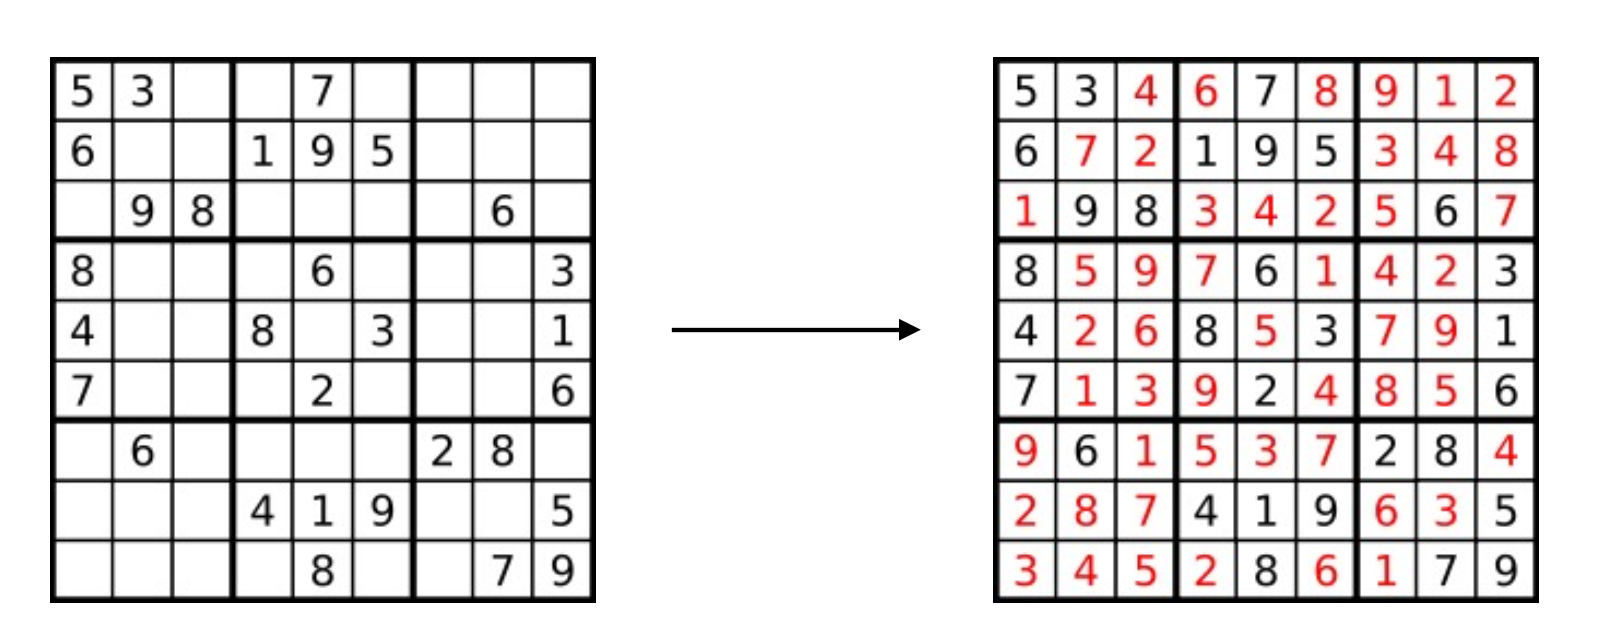
\includegraphics[width=0.7\linewidth]{images/lc0037_example}
	\label{fig:lc0037example}
\end{figure}
\begin{lstlisting}
board = [[ "5", "3", ".", ".", "7", ".", ".", ".", "." ], 
				 [ "6", ".", ".", "1", "9", "5", ".", ".", "." ],
				 [ ".", "9", "8", ".", ".", ".", ".", "6", "." ], 
				 [ "8", ".", ".", ".", "6", ".", ".", ".", "3" ],
				 [ "4", ".", ".", "8", ".", "3", ".", ".", "1" ], 
				 [ "7", ".", ".", ".", "2", ".", ".", ".", "6" ],
				 [ ".", "6", ".", ".", ".", ".", "2", "8", "." ], 
				 [ ".", ".", ".", "4", "1", "9", ".", ".", "5" ],
				 [ ".", ".", ".", ".", "8", ".", ".", "7", "9" ]]
				
output = [[ "5", "3", "4", "6", "7", "8", "9", "1", "2" ],
				  [ "6", "7", "2", "1", "9", "5", "3", "4", "8" ],
				  [ "1", "9", "8", "3", "4", "2", "5", "6", "7" ],
				  [ "8", "5", "9", "7", "6", "1", "4", "2", "3" ],
				  [ "4", "2", "6", "8", "5", "3", "7", "9", "1" ],
				  [ "7", "1", "3", "9", "2", "4", "8", "5", "6" ],
				  [ "9", "6", "1", "5", "3", "7", "2", "8", "4" ],
				  [ "2", "8", "7", "4", "1", "9", "6", "3", "5" ],
				  [ "3", "4", "5", "2", "8", "6", "1", "7", "9" ]]
\end{lstlisting}